\section{System architecture}
\label{sec:systemarchitecture}
\subsection{Overview}
The implementation uses a LangGraph directed graph with five specialised roles and a shared typed state. Indicator, Pattern, Trend and Decision roles, shared state, chart tools and trendline procedures reuse or modify QuantAgent components; the upstream MIT notice is preserved in the repository \cite{xiong2025quantagent}. Alpha adds numerical factor and Vietnamese sentiment reports. This integration is an engineering adaptation, distinct from inventing the inherited graph or validating a learned knowledge-fusion method.

Figure~\ref{fig:flow} shows the actual information flow. In the evaluated backtest, Indicator is deterministic and the numerical/report Alpha path bypasses an additional alpha-reasoning LLM call. Pattern and Trend consume their separate chart images, while Decision receives the condensed reports and enabled quantitative/text sections. The five role names consequently do not imply five hosted LLM calls per forecast. Model aliases and actual request accounting are specified in Section~\ref{sec:experimentalsetup}.

\begin{figure}[!htbp]
\centering
% Sơ đồ vai trò thực chạy; không biểu diễn learned fusion hoặc causal gate đã đạt.
\begin{tikzpicture}[
  role/.style={draw,rounded corners,align=center,text width=2.6cm,minimum height=0.85cm,font=\small},
  link/.style={-{Latex[length=2mm]},thick}]
\node[role,fill=gray!10] (price) at (0,-1.3) {Frozen OHLCV\\600-bar prefixes\\45-bar charts};
\node[role,fill=gray!10] (news) at (0,-3.9) {Frozen news scores\\Domain/PIT validity\\not established};
\node[role] (ind) at (4,0) {Indicator\\Deterministic report};
\node[role] (pat) at (4,-1.3) {Pattern\\Vision report/replay};
\node[role] (trend) at (4,-2.6) {Trend\\Corrected chart/report};
\node[role] (alpha) at (4,-3.9) {Alpha role\\Numeric factors and\\sentiment context};
\node[role,fill=blue!5,minimum height=1.6cm] (prompt) at (8,-1.9) {Shared I/P/T reports\\Enabled sections\\Heuristic prompt\\instructions};
\node[role] (decision) at (12,-1.9) {Decision LLM\\Structured LONG\\or SHORT};
\node[role,fill=gray!10] (ledger) at (12,-3.9) {Account simulation\\SHORT maps to CASH};
\draw[link] (price.east) -- (ind.west);
\draw[link] (price.east) -- (pat.west);
\draw[link] (price.east) -- (trend.west);
\draw[link] (price.east) -- (alpha.west);
\draw[link] (news.east) -- (alpha.west);
\draw[link] (ind.east) -- (prompt.west);
\draw[link] (pat.east) -- (prompt.west);
\draw[link] (trend.east) -- (prompt.west);
\draw[link,dashed] (alpha.east) -- (prompt.south west);
\draw[link] (prompt.east) -- (decision.west);
\draw[link] (decision.south) -- (ledger.north);
\node[align=center,font=\small,text width=4.3cm] at (8,-3.9) {Base omits factor and sentiment sections;\\no learned fusion module};
\end{tikzpicture}

\caption{System pipeline with shared-report Full/Base comparison. Indicator and alpha backtest reports are deterministic/numerical; Pattern and Trend use vision requests. Decision aggregates enabled reports by prompt instructions.}
\label{fig:flow}
\end{figure}

\subsection{Indicator Agent}
Indicator Agent computes and renders five deterministic TA-Lib-based votes: MACD(12,26,9), RSI(14), Stochastic(14,3,3), Williams \%R(14) and ROC(10). They are momentum/trend indicators, not five volatility oscillators. Its backtest node returns a report and messages, without calling an LLM or forwarding the declared state schema's complete numeric arrays. Bollinger variables can be computed on the alpha path; BB/ADX state declarations do not create two additional Indicator votes. \ref{app:indicator_logic} specifies the ordered boundaries and missing-data convention \cite{talib_rsi_docs,talib_willr_docs}.

Four-decimal rounding precedes classification, nonfinite samples are removed and zero is retained. Crossovers take priority where specified; overlapping RSI/Williams thresholds require ordered branches rather than two simultaneous unconditional rules. Each missing/error result contributes a neutral vote within the fixed denominator of five. Directional plurality and the confidence categories are deterministic summary heuristics. They are not calibrated probabilities, and an immutable signal tally does not make a downstream narrative correct.

\subsection{Alpha Agent}
\paragraph{Alpha selection}
The Alpha role evaluates 85 native candidates: 80 retained WorldQuant adaptations and five custom formulas. It supplies a selected top-five report from the trailing prefix, using the diagnostic score in Eq.~\ref{eq:composite}. The transformations, metric support, IC orientation and native row-wise causal failure are defined in Section~\ref{sec:formulation}. A rolling own-history rank is not a cross-sectional rank, and the 21 exclusions are not all justified by an inability to translate cross-sectional operators. Full expressions and exception handling remain in the registry; \ref{app:signals} gives the custom formulas needed to read the reports.

Selection, IC sign and candidate diagnostics reuse trailing observations. Hence the current value is an input to a report, while the reported skill fields are in-sample ranking statistics. Neither choosing the top five nor reversing negative IC establishes out-of-sample profitability. Six selected metadata slots have description/handler mismatches; actual prompts, metadata and implementation identity are kept distinct. No historical prediction is repaired to agree with a corrected description.

\paragraph{Sentiment integration}
Vietnamese sentiment is a separate contextual report, not an input to the native OHLCV factor formulas or score. The frozen provider supplies aggregate/count information and empty article-detail/peer lists. Relative sentiment and z-score fields on that path are consequently zero-valued outputs of the normalizer, rather than measured contemporaneous peer evidence. The three-article availability rule differs from the eight-article reliability flag. The 90-day window, 30-day decay, scorer revision and provenance limitations are specified in Section~\ref{sec:formulation}.

Figure~\ref{fig:alpha_agent} separates OHLCV factor selection from sentiment-context construction and shows the information delivered by the evaluated backtest. Optional live endpoints, lexicon fallbacks and peer discovery are repository capabilities; they are not evidence that the corresponding inputs were used or historically available in the evaluated calls.

\begin{figure}[!htbp]
\centering\begin{tikzpicture}[x=1cm,y=1cm,>=Latex,
 box/.style={draw=blue!55!black,fill=blue!4,rounded corners,align=center,text width=6.4cm,minimum height=1.2cm,font=\footnotesize},
 sent/.style={box,draw=green!40!black,fill=green!4},
 endbox/.style={draw=orange!65!black,fill=orange!7,rounded corners,align=center,text width=13.7cm,minimum height=1.2cm,font=\footnotesize},
 arr/.style={->,thick}]
\node[font=\bfseries] at (0,1.1) {Native OHLCV path};
\node[font=\bfseries] at (7.3,1.1) {Separate frozen sentiment path};
\node[box] (a1) at (0,0) {Prefix ending at decision $d$\\Up to 600 observed bars};
\node[box] (a2) at (0,-1.8) {85 native candidates\\80 adaptations + five custom handlers};
\node[box] (a3) at (0,-3.6) {Finite-support diagnostics and IC sign\\Same trailing sample; in-sample selection};
\node[box] (a4) at (0,-5.4) {Weighted score; select top five\\Native row-wise causal defect remains};
\node[box] (a5) at (0,-7.2) {Factor report / skill fields\\Compact or explicit-five-row family};
\node[sent] (s1) at (7.3,0) {Saved article scores and provenance\\Historical availability unverified};
\node[sent] (s2) at (7.3,-1.8) {90-day cutoff window; distinct identities\\At least three valid records for availability};
\node[sent] (s3) at (7.3,-3.6) {Probability difference / weighted mean\\30-day decay half-life};
\node[sent] (s4) at (7.3,-5.4) {Aggregate/count report\\No observed peer/article-detail comparison};
\node[sent] (s5) at (7.3,-7.2) {Separate sentiment text / missingness\\Reliability $\ge8$ is a different flag};
\node[endbox] (o) at (3.65,-9.3) {Variant-enabled sections enter Decision; sentiment does not enter native factor formulas.\\No extra Alpha reasoning-model call on this backtest path.};
\foreach \p/\q in {a1/a2,a2/a3,a3/a4,a4/a5,s1/s2,s2/s3,s3/s4,s4/s5}{\draw[arr] (\p)--(\q);}
\draw[arr] (a5.south)--(a5.south |- o.north);
\draw[arr] (s5.south)--(s5.south |- o.north);
\end{tikzpicture}

\caption{Alpha Agent: native OHLCV selection and separate sentiment context. Native factor diagnostics retain their causal/selection defects; the frozen sentiment path has no authenticated peer comparison. Both reports enter Decision only when enabled by the variant.}
\label{fig:alpha_agent}
\end{figure}

\subsection{Pattern Agent}
Pattern Agent analyses a candlestick PNG rendered from the exact 45-bar window. The prompt requests a chart formation, recent-candle evidence, directional bias, confidence and trading implication. The report parser retains the structured text fields; format completion and consistency checks are distinguished from financial correctness. Figure~\ref{fig:charts} presents an actual archived chart pair rather than a synthetic demonstration.

Candle bodies are green when Close exceeds Open and red otherwise, including a doji. This is an Open--Close body rule, not the Vietnamese exchange board's reference-price colouring rule. The exchange-board convention is not used to infer candle direction. After inference, consistency rules compare the claimed bias with simple OHLCV-derived properties such as the final body and recent closes. A contradiction flag can reduce displayed confidence; it cannot reveal which candle the VLM actually attended to. Alternative text-only paths in the general application are not assumed to have replaced any frozen vision input.

\begin{figure}[!htbp]
\centering
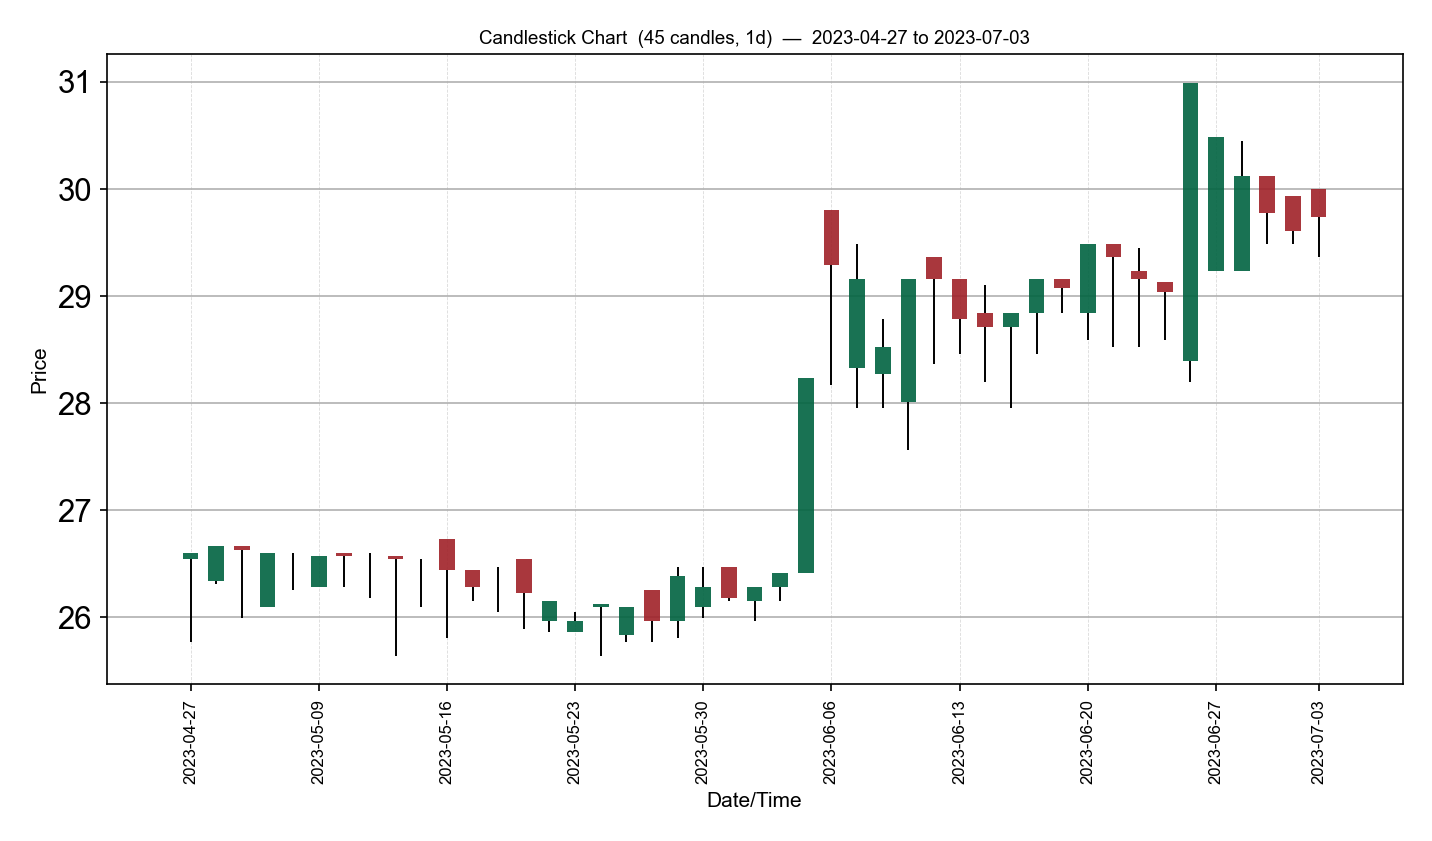
\includegraphics[width=0.90\textwidth]{figs/final_pattern.png}\par\smallskip
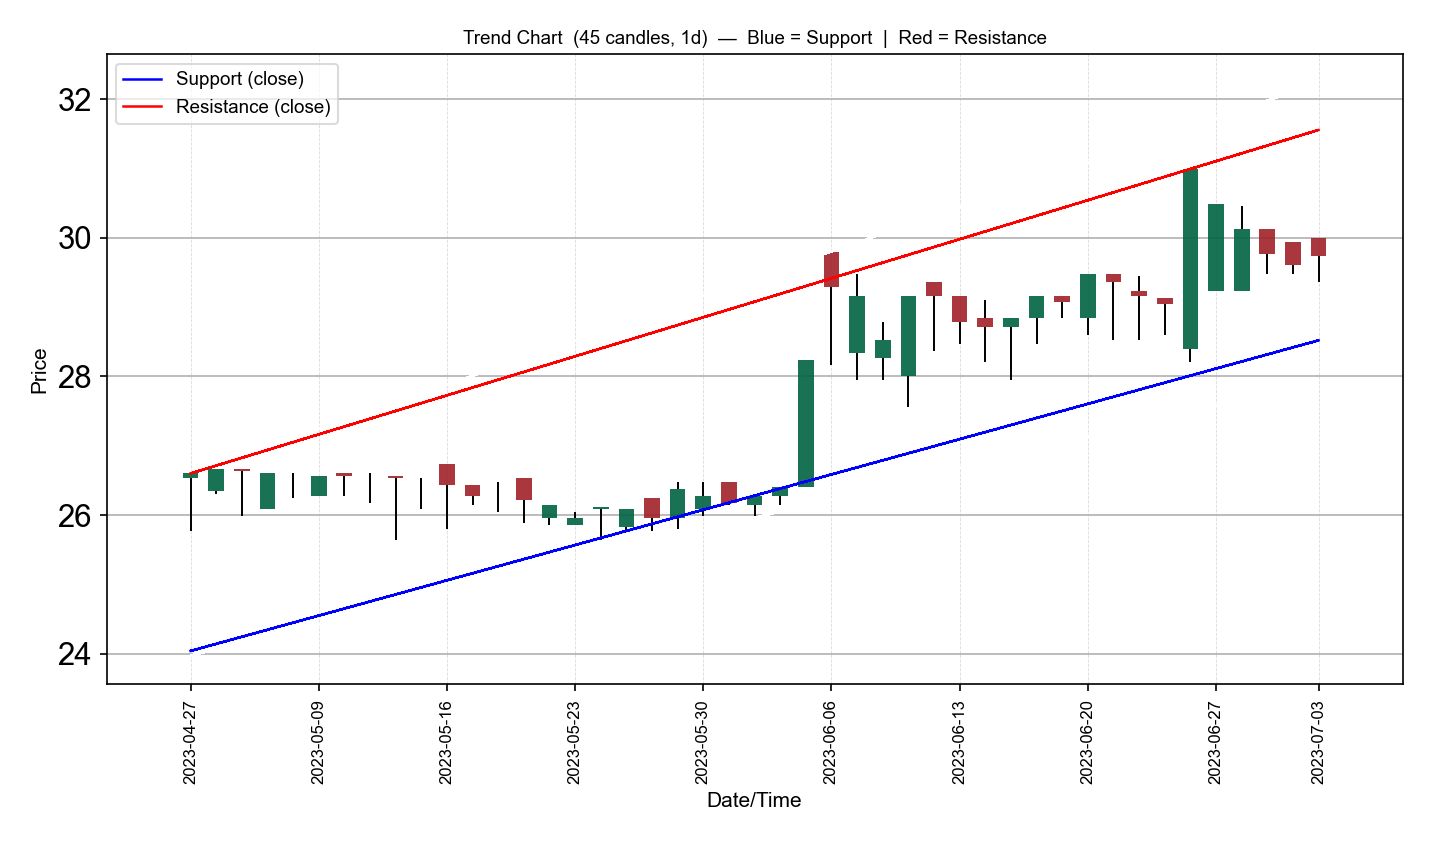
\includegraphics[width=0.90\textwidth]{figs/final_trend.png}
\caption{Actual Pattern and corrected Trend inputs for CMG on 3 July 2023, the first chronologically eligible main unit. Bodies compare Close with Open; the Trend legend maps blue to support and red to resistance. The unit was selected by date then symbol/ID without inspecting outcomes.}
\label{fig:charts}
\end{figure}

\subsection{Trend Agent}
Trend Agent receives a separate chart with fitted support/resistance lines. The inherited fitting utility starts with a least-squares close-price line, selects upper/lower deviation pivots, and optimizes a slope through each pivot under a non-crossing constraint. It implements both a close-only channel and a high/low channel, the latter using close-price regression to find pivots and high/low data for the bounds. These are numerical lines over the supplied window, not human-verified latent support levels.

For row position $u$, a fitted line has form $b+mu$. A support bound must remain below the corresponding price sequence within the implementation tolerance; resistance must remain above it. The local slope search reduces its step when the squared-deviation objective fails to improve or violates the constraint. The VLM then describes direction, levels, slope, price relative to support, forecast and confidence. Support is drawn blue and resistance red. A deterministic consistency check against simple price/trend summaries does not validate every reported level or coordinate.

The renderer audit matched 204 images across 102 units byte for byte and pixel for pixel, and 240 actual vision requests matched their image caches and Vietnamese templates. It verified body geometry, colour and legend handles, not the model's visual understanding. In particular, the Vietnamese word \emph{xanh} is less colour-specific than the corrected English ``blue'' wording. Inherited high-frequency/K-line prompt language also remains distinguishable from this daily-bar application. Matched local-pattern interventions and trend swaps would be needed to test whether the model uses the purported visual evidence.

\subsection{Decision Agent}
Decision receives condensed Indicator, Pattern and Trend reports plus enabled factor/sentiment sections. Reports are distilled and capped before prompt composition. The observed successful Decision prompts are at most 4,187 characters, below the 6,500-character guard. Figure~\ref{fig:decision_agent} shows report composition, prompt instructions, structured output and the separate action mapping.

\begin{figure}[!htbp]
\centering\begin{tikzpicture}[x=1cm,y=1cm,>=Latex,
 box/.style={draw=blue!55!black,fill=blue!4,rounded corners,align=center,text width=6.5cm,minimum height=1.8cm,font=\footnotesize},
 act/.style={box,draw=orange!65!black,fill=orange!6},arr/.style={->,thick}]
\node[box] (r) at (0,0) {\textbf{1. Shared reports}\\Indicator / Pattern / Trend\\Enabled factor/sentiment text};
\node[box] (p) at (7.6,0) {\textbf{2. Distil and compose prompt}\\Observed maximum: 4,187 characters\\Guard: below 6,500 characters};
\node[box] (i) at (0,-2.9) {\textbf{3. Evidence-priority instructions}\\Trend/candles; then momentum\\Enabled factors and sentiment};
\node[box] (j) at (7.6,-2.9) {\textbf{4. Structured forecast}\\LONG/SHORT; horizon; confidence\\Risk/reward; evidence; justification};
\node[act] (l) at (0,-5.8) {\textbf{LONG: reference action}\\Buy at next Open; exit at target Close\\Both-leg brokerage and slippage};
\node[act] (c) at (7.6,-5.8) {\textbf{SHORT: CASH action}\\No short sale or bearish return\\DOWN remains a classification};
\draw[arr] (r)--(p);
\draw[arr] (p.south)--++(0,-0.5)-|(i.north);
\draw[arr] (i)--(j);
\draw[arr] (j.south)--++(0,-0.5)-|(l.north);
\draw[arr] (j.south)--(c.north);
\node[align=center,text width=14.0cm,font=\footnotesize] at (3.8,-7.8) {Prompt precedence and model confidence are heuristics; they do not certify reasoning,\\calibration, executable fills or a learned fusion mechanism.};
\end{tikzpicture}

\caption{Decision Agent pipeline. Evidence priorities are prompt heuristics rather than learned/calibrated weights. The structured forecast is evaluated separately from the conditional long-only account action.}
\label{fig:decision_agent}
\end{figure}

The instructions ask for trend/key-level assessment, recent-candle evidence, momentum confirmation and comparison with enabled factor/sentiment context. Price/chart evidence has priority, quantitative factors may challenge it, and sentiment has lower priority. These instructions describe an intended analysis sequence; they are not an independently observed internal reasoning trace or a guaranteed conflict-resolution algorithm.

The required output includes a binary LONG/SHORT forecast, forecast horizon, confidence, risk/reward field, evidence for/against and justification. Model confidence and risk/reward statements do not constitute calibrated uncertainty or executable price levels. In the long-only reference ledger, SHORT maps to CASH and LONG to the specified next-open/target-close cycle. The classifier's labels and account execution remain distinct.

Base retains the same upstream content and general instructions but removes both alpha and sentiment sections; those concepts may still appear in general instructions. Thus Full--Base changes a bundle and prompt length, not solely one numerical factor. Main/upstream prompts use compact factor text, whereas factorial A/AS/P deliver five explicit rows. The resulting representation difference remains part of the interpretation of the separate panels.
